\documentclass[10pt,draftclsnofoot,onecolumn,journal,compsoc]{IEEEtran}

\usepackage[margin=0.75in]{geometry}
\usepackage{graphicx}
\usepackage{caption}
\usepackage{hyperref}
\usepackage{enumerate}
\usepackage{tabu}
\usepackage[english]{babel}\usepackage[numbers]{natbib}
\usepackage{natbib}
\usepackage{longtable}
\usepackage{listings}
\usepackage{pgfgantt}
\usepackage{vhistory}

\renewcommand{\linespread}{1.0}
\renewcommand{\bibsection}{}

\lstset{
captionpos=b,           
}

\renewcommand{\linespread}{1.0}
\title{Prototype Big Data Archive in a Public Cloud}
\author{
  \IEEEauthorblockN{Group 56: Pathfinder of Big Data\\Zhi Jiang, Isaac T Chan, Zhaohensg Wang} \\
  \IEEEauthorblockA{CS 461: Senior Capstone Fall 2016 \\ Oregon State University}
}
\date{}

\IEEEtitleabstractindextext{
	\begin{abstract}
OSU campuses generate data constantly from multiples sources, including computer labs, wireless usage, student devices, and many others. This quantity of data, also known as big data which will effectively represent all kinds of behaviors of students for information technology. However, the data is very difficult to manage because it is collected from multiple sources and is hard to analyze. As a result, various technologies will be required for supporting this project. In this document, we will talk about these technologies based on different viewpoints such as context, information or algorithm. For each viewpoint, we will declare the design concerns for it. Besides, we will introduce our technology detail based on these viewpoints.
	\end{abstract}
}


\begin{document}
% cover page    
    \maketitle
    \IEEEdisplaynontitleabstractindextext
    \IEEEpeerreviewmaketitle
    \newpage
% catalog    
    \tableofcontents
    \newpage

% revision history
	\begin{versionhistory}
  \vhEntry{1.0}{2017.02.06}{Zhi Jiang}{created revision history}
  \vhEntry{1.1}{2017.02.07}{Zhi Jiang}{modified the time line}
\end{versionhistory}
	\newpage

% content   
\section{Introduction}
	\section{Introduction}
	\subsection{Purpose}
    OSU campuses generate data constantly from multiples sources, including computer labs, wireless usage, student devices, and many others. This quantity of data, also known as big data, can effectively represent student behaviors for information technology. For example, analysis can be run to determine common student behaviors in order to allocate OSU resources to more often used utilities. Currently, the data is very difficult to manage because it is collected from multiple sources and is impossible to analyze. The data is neither stored in the same formats nor in the same locations, meaning it is inaccessible and useful information is unable to be extracted. The purpose of this project is to unify the data onto the consistent cloud platform of Amazon Web Services, which additionally provides utilities to manage and analyze.
    
    \subsection{Current Position}
    Currently, the functional part of the project is complete. We have a working database implementation in the Amazon Web Services public cloud, with appropriate storage, loading, and restricted access for sensitive data. By leveraging additional services in the AWS environment, we are able to provide rudimentary analysis, reporting, and visualization of data. From this position, we are able to present at Expo on the entire project, from beginning to end, including potential outcomes if the project were adopted by OSU. In the original project description, there were three deliverables listed. We have completed two of them: the database implementation and analysis/reporting/visualization. The third, a cost model, has yet to be complete. In order to provide an accurate cost model, we require an estimate for data amounts and are currently waiting for the estimate. This deliverable won't affect the project demonstration at Expo and is soley for the benefit of our client to decide on whether OSU will adopt our prototype.

\section{References}
	\begin{thebibliography}{1}
%Issac    
        \bibitem{I1}G. Kamat, "YCSB, the Open Standard for NoSQL Benchmarking, Joins Cloudera Labs", \textit{Cloudera}, 2015. Available: http://blog.cloudera.com/blog/2015/08/ycsb-the-open-standard-for-nosql-benchmarking-joins-cloudera-labs/. [Accessed: 14- Nov- 2016].
        
        \bibitem{I2}"TPC-H - Homepage", \textit{Tpc.org}, 2016. [Online]. Available: http://www.tpc.org/tpch/. [Accessed: 14- Nov- 2016].
%Zhi        
        \bibitem{Z1}M. Nemschoff, "Big data: 5 major advantages of Hadoop", \textit{IT Pro Portal}, 2013. [Online]. Available: http://www.itproportal.com/2013/12/20/big-data-5-major-advantages-of-hadoop/. [Accessed: 14- Nov- 2016].
        
        \bibitem{Z2}"What is Hadoop?", \textit{Amazon Web Services}, Inc., 2016. [Online]. Available: https://aws.amazon.com/emr/details/hadoop/?nc1{$=$}h\_ls. [Accessed: 14- Nov- 2016].
        
        \bibitem{Z3}S. Neumann, "Storing Apache Hadoop Data on the Cloud - HDFS vs. S3", \textit{Xplenty.com}, 2014. [Online]. Available: https://www.xplenty.com/blog/2014/03/storing-apache-hadoop-data-cloud-hdfs-vs-s3/. [Accessed: 14- Nov- 2016].
        
        \bibitem{Z4}L. Joseji, "6 Sparkling Features of Apache Spark!", \textit{dzone.com}, 2014. [Online]. Available: https://dzone.com/articles/6-sparkling-features-apache. [Accessed: 14- Nov- 2016].
        
        \bibitem{Z5}S. Neumann, "Spark vs. Hadoop MapReduce", \textit{Xplenty.com}, 2014. [Online]. Available: https://www.xplenty.com/blog/2014/11/apache-spark-vs-hadoop-mapreduce/. [Accessed: 14- Nov- 2016].
        
        \bibitem{Z6}"Amazon Kinesis Streams", \textit{Amazon Web Services, Inc.}, 2016. [Online]. Available: https://aws.amazon.com/kinesis/streams/?nc1{$=$}h\_ls. [Accessed: 14- Nov- 2016].
        
        \bibitem{Z7}"Apache Hive - Amazon EMR", \textit{Docs.aws.amazon.com}, 2016. [Online]. Available: http://docs.aws.amazon.com/ElasticMapReduce/latest/ReleaseGuide/emr-hive.html. [Accessed: 14- Nov- 2016].
        
        \bibitem{Z8}Amazon EMR - Developer guide. \textit{Amazon Web Services, Inc.}. [Online]. Available: http://docs.aws.amazon.com/ElasticMapReduce/latest/DeveloperGuide/emr-dg.pdf. [Accessed: 14- Nov- 2016].
        
%Zhaoheng        
        \bibitem{W1}"Why you probably shouldn't use cookies to store session data", \textit{Wonko.com}, 2008. [Online]. Available: http://wonko.com/post/why-you-probably-shouldnt-use-cookies-to-store-session-data. [Accessed: 14- Nov- 2016].
        
        \bibitem{W2}S. Knickelbine"Benefits of Using a Database", \textit{Work.chron.com}, 2016. [Online]. Available: http://work.chron.com/benefits-using-database-3792.html. [Accessed: 14- Nov- 2016].
        
        \bibitem{W3}"Advantages of Database", \textit{Ecomputernotes.com}, 2016. [Online]. Available: http://ecomputernotes.com/fundamental/what-is-a-database/advantages-of-database. [Accessed: 14- Nov- 2016].
        
        \bibitem{W4}D. Thakur"SQL vs NoSQL Database Differences Explained with few Example DB", \textit{Thegeekstuff.com}, 2016. [Online]. Available: http://www.thegeekstuff.com/2014/01/sql-vs-nosql-db/?utm\_source$=$tuicool. [Accessed: 14- Nov- 2016].
        
        \bibitem{W5}"Amazon DynamoDB Product Details", \textit{Amazon Web Services, Inc.}, 2016. [Online]. Available: https://aws.amazon.com/dynamodb/details/?nc1{$=$}h\_ls. [Accessed: 14- Nov- 2016].
        
        \bibitem{W6}"Amazon QuickSight Business Intelligence Software", \textit{Amazon Web Services, Inc.}, 2016. [Online]. Available: https://aws.amazon.com/quicksight/. [Accessed: 14- Nov- 2016].
    \end{thebibliography}

\section{Glossary}
	\section{Glossary}
\begin{tabu} to \hsize {|X|X[2,l]|}
        \hline
        \textbf{Term} & \textbf{Definition}\\
        \hline
        User & People who interact with our project \\
        \hline
        DB & Database\\
        \hline
        Nosql & Non-relational database\\
        \hline
        SDK & Software development kit\\
         \hline
        Schema & Database table \\
        \hline
        AWS & Amazon web service, a Platform as a service(PaaS) offered by Amazon \\
        \hline
        S3 & Simple storage service provided by Amazon\\
        \hline
        Amazon Kinesis & A service used to process stream and log file data \\
        \hline
        SQL & a standard programming language used to access and process database or data storage\\
        \hline
        EC2 & a web service that provides resizable compute capacity in the cloud\cite{g1}\\
        \hline
        EMR & A comprehensive tool that can manage data and provide analysis through conventional queries or machine learning technology\\
		\hline
\end{tabu}

\section{Timeline}
	\begin{ganttchart}[vgrid, hgrid]{1}{18}
        \gantttitle{Winter}{10}
        \gantttitle{Spring}{8}\\
        
        \gantttitlelist{1,...,10}{1}
        \gantttitlelist{1,...,8}{1}\\
        
        \ganttbar{Data storage implementation}{1}{1}\\ 
        \ganttbar{Database table implementation}{1}{2}\\
        \ganttbar{Application of parsing data}{2}{4}\\
        \ganttbar{Application of transforming data}{4}{6}\\
        \ganttbar{Data visualization}{7}{8} \\
        
        \ganttbar{Test for functionality}{9}{11} \\
        \ganttbar{Performance optimization}{10}{13}\\
        \ganttbar{Security optimization}{13}{16}\\
        \ganttbar{Cost comparison}{17}{18}
 \end{ganttchart}
    
%body
\section{AWS Cloudwatch}
    \subsection{Context}
    Performance metrics for database functionality is an important element of the implementation. We will assess performance from typical database operations: data inserts, updates, and reads. After reviewing different technologies, AWS Cloudwatch is the utility we will use to perform these operations and measure the performance.
    
    \subsection{Viewpoint: Users}
    We will have one primary user for the implemented system: OSU staff who perform data analysis. From their viewpoint, performance is an incredibly important feature of the database. The data analyzer may be performing analysis on potentially extremely large data sets; if the speed of reading the data in the database is slow, it is not a successful implementation. We understand that “slow” is a vague term, but without a method of comparison it is impossible to judge the collected performance metrics as of now. We will meet with current data analyzers and our client to determine whether or not the performance meets expectations.\\
    
    \noindent In order to accurately provide a model for realistic usage, we will need to measure performance of database operations using differing sizes of sample data.
    
    \subsection{Viewpoint: Scalability}
    Another large aspect of our database implementation is the ability for it to scale well in the future, with more and more data added. Although this will of course affect the user, scalability will also affect the database administrator. Performance for inserting and updating data within the database is directly related to scalability, and whether or not the performance is heavily affected by the amount of stored data.\\
    
    \noindent We will use large sets of sample data to load into the database. These large sizes should again, differ in size in order to model an estimation for future database performance.
    
    \subsection{Implementation}
    In AWS Cloudwatch, we will utilize the built-in PutMetricData API to input custom metrics for Cloudwatch to monitor\cite{i1}. This API works by passing measurements of interest into the API and the measurements are saved to a location within AWS for us to view.\\
    
	\noindent Here is a code example of checking CPU utilization, using the Cloudwatch command line interface. As shown, it displays the namespace, as well as the runtime. After collecting these types of metrics using differing sizes of data, we can provide an accurate model and estimate projected metrics with extremely large data sets.

\begin{lstlisting}[caption=Cloudwatch monitoring example\cite{i2}]
mon-get-stats CPUUtilization   
      --namespace="AWS/RDS"     
      --dimensions="DBInstanceIdentifier=instance-name"
      --statistics Maximum
      --start-time 2015-09-29T00:00:00   
      --end-time 2015-09-29T00:05:00
\end{lstlisting}

\section{Database Security}
	\subsection{Context}
    With methods database security, we hope to improve the security of our database by restricting access and preventing malicious utilization of data. Our best options for database security is AWS’s user authentication policies, encrypting sensitive data fields, and using sufficient input validation to avoid injection attacks.
    \subsection{Viewpoint: Users}
    From a data analyzer viewpoint, database security is a concern, in order to prevent unintended data loss, either from malicious users or unfortunate accidental injection attacks. Data loss, if unrecognized while performing analysis, can result in incorrect conclusions drawn from incomplete data. Additionally, waiting for backups to be restored or missing data to be re-inserted takes up time and hinders work.
    
    \subsection{Adminstrators}
    From an administration perspective, database security is a concern to reduce the possibility of malicious user access. Administrators will carefully restrict the number of authenticated users using AWS’s user authentication policies. Most of the data inside the database is OSU’s system users, with identifying fields such as student ID’s. If a malicious user were to gain access to the database, it would be a massive privacy breach for them to have access to identifying features of such high volume. Administrators will encrypt these identifying fields to prevent identification of the data.\\
    
    \noindent Elements of course include the database and subsequent data. Additionally, after we assess the necessity of including backups, possibly backups. 
    
    \subsection{Implementation}
    AWS’s user authentications, also known as AWS IAM (Identity and Access Management), is quite robust. Administrators can create and manage AWS users and groups, while setting permissions to restrict access to certain AWS resources\cite{i3}. For example, administrators can set modularize groups to only have access to data ingestion, processing, or database for analysis. This prevents a large number of users to have access to the whole system and increases liability and responsibility for the users.\\
    
	\noindent As we implement the database, the user-identifying fields within the data is already encrypted to protect us as developers and reduce liability for our client. This encryption will remain within the database and future data inserts will be encrypted as according to the administrators.\\
    
	\noindent Finally, minimizing possibility of injection attacks. There is inherent protection when user authentication is done properly, because authenticated users will not be as likely to perform malicious operations. However, we will be implementing our NoSQL database with AWS DynamoDB, which inherently prevents injection attacks by not allowing multiple operations within one command.
    
\section{User Interaction}
	\subsection{Context}
    Users will need to be able to interact with the system. They will need to use different utilities for different interactions, such as monitoring resources, monitoring performance, managing data, and performing different methods of analysis. As discussed previously regarding performance metrics, the utility of choice for monitoring is AWS Cloudwatch. For the different methods of analysis, we chose AWS EMR as the most well-rounded utility for comprehensive coverage of analysis techniques.
    
    \subsection{Viewpoint: Data analyzers}
    From the viewpoint of a data analyzer, they will be of course interested mainly in performing analysis on the data within the database. It is their choice what utility they use, but as the developers we would like to ensure the database implementation is acceptable. We chose AWS EMR as the utility we will test our database with. From EMR, we can perform basic tests to ensure data analysis is possible.\\ 
    
    \noindent AWS EMR is a managed Hadoop framework in a command line interface\cite{i4}. Scripts and code can be run from AWS EMR. As developers, we will be running basic data analysis code from EMR against the implemented database to ensure analysis is possible.
    
    \subsection{Viewpoint: Administrators}
    From an administrative perspective, they will be interacting with the system with monitoring and management utilities. Because monitoring was covered in-depth in the performance metrics section, this section will mainly be on the management utility. Database management includes operations such as inserting new or updating data within the database. This can be achieved using our database implementation utility, AWS DynamoDB. See section 10, DynamoDB for more details.
    
    \subsection{Implementation}
    Provided is a sample python script to perform a linear regression analysis on a set of data. Obviously as of now, the analysis is purely hypothetical, considering we do not currently have a source of data, nor we do know how the data will be analyzed. This sample code is only a proof of concept that scripts such as these can be run within AWS EMR to ensure analysis is possible with our database implementation.
    
\begin{lstlisting}[caption=Sample EMR linear regression analysis example\cite{i5}]
def fit(X, Y):

    def mean(Xs):
        return sum(Xs) / len(Xs)
        
    m_X = mean(X)
    m_Y = mean(Y)

    def std(Xs, m):
        normalizer = len(Xs) - 1
        return math.sqrt(sum((pow(x - m, 2) for x in Xs)) / normalizer)

    def pearson_r(Xs, Ys):
        sum_xy = 0
        sum_sq_v_x = 0
        sum_sq_v_y = 0

        for (x, y) in zip(Xs, Ys):
            var_x = x - m_X
            var_y = y - m_Y
            sum_xy += var_x * var_y
            sum_sq_v_x += pow(var_x, 2)
            sum_sq_v_y += pow(var_y, 2)
        return sum_xy / math.sqrt(sum_sq_v_x * sum_sq_v_y)

    r = pearson_r(X, Y)
    b = r * (std(Y, m_Y) / std(X, m_X))
    A = m_Y - b * m_X

    def line(x):
        return b * x + A
    return line
\end{lstlisting}
\section{S3}
	\subsection{Context}
	The purpose of S3, as a data storage, is used to store all files, and these files include unformatted and uncleaned data and results integrated into analytics tool. S3 gains any types of data and format data from the user and then move them to other services in Amazon platform.
        
	\subsection{Composition}
	\begin{itemize}
		\item \textbf{Buckets:} bucket is a basic container used to store objects in S3.\cite{z1}
		\item \textbf{Objects:} Objects are the fundamental entities stored in S3, and it consists of object data and metadata. The role of metadata is to store set of name-value pairs that describe the object.\cite{z1}
		\item \textbf{Keys:} each object has the unique identifier and which is called “key”. In order to ensure uniqueness of each object, the combination of a bucket, key and version ID is used to identify each object in S3.\cite{z1}
	\end{itemize}

	\subsection{Interaction}
    S3 need to upload data to analytics and send data to database, thus S3 will interact with the Data Pipeline, and then complete data transforming between different compute and storage services according to the application on data pipeline. On the other hand, the developer needs to program some functions for S3, thus S3 will interact with AWS Lambda. The role of AWS Lambda is to run code for all backed services on this platform.
    
	\subsection{Algorithm}
    The AWS SDK supports several programming languages to develop S3 by programming. The programming languages cover Java, .NET, Ruby, Python and PHP. On the other AWS SDK also provide many API for these programming languages. Take an instance with Java, the developer can utilize low-level API to implement create, update, and delete operations that apply to buckets and objects in S3.\cite{z2} 

 \section{AWS SDK for Python}
	\subsection{Context}
    The role of AWS SDK for Python is to complete all operations for data from S3 such as integrating data, parsing data and transferring data. These operations can ensure consistency and normalization of data which will be moved to the database.  
        
	\subsection{Dependency}
    This tool is not completely independent from others because the Python script must be compiled on a service. Another Amazon Web Service EC2 as the cloud-computing platform can help the developer to compile it. 
    
	\subsection{Interaction}
    AWS SDK for Python must interact with other entities. There are two reasons. One is this portion needs to receive data from other services. Second reason is the results should be exported to other services after data parsed by the Python script.

	\subsection{Algorithm}
    The core concept of AWS SDK for Python is to help developers creating one or more applications related Amazon services like S3 and DynamoDB. Boto 3 is the AWS SDK for Python and it is able to provide enough methods to solve some general problems between these services.
    
	\begin{itemize}
	\item \textbf{Accessing S3:} 
	The purpose of accessing S3 service is to gain data we want to process from it. S3 as a data storage stores all source files, so accessing S3 service is the first step in our project. The Boto 3 provides higher-level resources for S3. Then, we need to get a specific bucket in an S3 resource. There is an example showing how to access S3 service and bucket into it.\\
	\begin{lstlisting}[language=Python, caption=Accessing S3 example\cite{z4}]
		import boto3
		
		# Get the S3 service resource.
		s3 = boto3.resource('s3')
		
		# Access the bucket ‘mybucket’ into S3
		bucket = s3.Bucket('mybucket')
	\end{lstlisting}	
	
	\item\textbf{Accessing DynamoDB:}
	The purpose of accessing DynamoDB is the results must be imported to a table into DynamoDB. The basic idea to access DynamoDB is similar to access S3. We need to access a specific table after we gain DyanmoDB resources. There is still an example of them:\\
	\begin{lstlisting}[language=Python, caption=Accessing DynamoDB\cite{z4}]
		import boto3
		
		# Get the DynamoDB service resource.
		dynamodb = boto3.resource('dynamodb')

		# Access the table ‘users’ into DynamoDB
		table = dynamodb.Table('users')
	\end{lstlisting}
	\end{itemize}
       
\section{Data Pipeline}
	\subsection{Context}
    The product relates to a number of different compute and storage services thus function of AWS Data Pipeline is to help user efficiently and massively move data among these services.
     
     \subsection{Composition}
     \textbf{Data node:} entity of data source in the pipeline, and attributes of it consist of name, locations, and formats\cite{z5}. 
     
     \noindent\textbf{Activity:} activity represents methods to transform data such as moving data from one location to another. 
     
     \noindent\textbf{Schedule:} each activity has own schedule for operating data
     
     \noindent\textbf{Resources:} entity that implements activities when they are scheduled 
     
	\subsection{Dependency}
	Data Pipeline must depend on other services because the main goal of it is to transform data from other data sources. On the other hand, the activities are extensible, so the developer is allowed to run custom scripts to implement more combinations.
     
    \subsection{Structure}
	The following diagram represents a complete structure of the Data Pipeline. 

    \begin{figure}[H]
        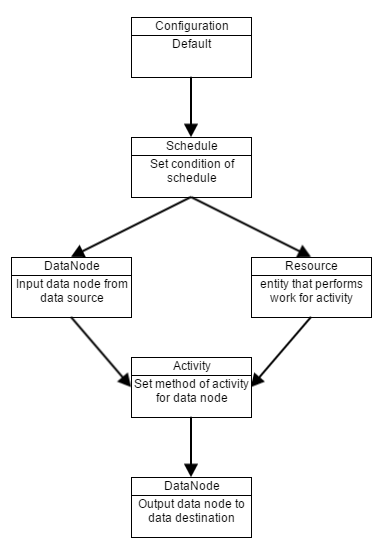
\includegraphics[width=10cm, height=14cm]{data_pipeline.png}
        \centering
        \caption{Complete structure of Data Pipeline}
    \end{figure}
    
	\subsection{Interaction}
	AWS provides management console to create a data pipeline directly. The developer can set the data source and data destination, and then the new data pipeline will automatically make  a connection between these two locations.  
    
	\subsection{Algorithm}
	In this product, the locations are S3 and DynamoDB for data pipeline, thus all of algorithms must be associated to these two services. AWS Data Pipeline supports \textbf{S3DataNode} and \textbf{DynamoDBDataNode}. The  object example of \textbf{S3dataNode} is

	\begin{lstlisting}[language=Java, caption=S3 Data Node example\cite{z6}]
        {
            "id" : "OutputData",
            "type" : "S3DataNode",
            "schedule" : { "ref" : "CopyPeriod" },
            "filePath" : "s3://myBucket/#{@scheduledStartTime}.csv"
        }
	\end{lstlisting}
	And the object example of \textbf{DynamoDBDataNode} is 
	\begin{lstlisting}[language=Java, caption=DynamoDB Data Node example\cite{z7}]
        {
            "id" : "MyDynamoDBTable",
            "type" : "DynamoDBDataNode",
            "schedule" : { "ref" : "CopyPeriod" },
            "tableName" : "adEvents",
            "precondition" : { "ref" : "Ready" }
        }
	\end{lstlisting}

	\noindent In term of algorithm of activity, AWS Data pipeline provides several general activities to accommodate common scenarios. These activities include \textbf{CopyActivity}, \textbf{HiveActivity}, \textbf{PigActivity}, etc.\\ 
    
    \noindent Resource is used to make these activities work on data node. The AWS Data Pipeline supports two kinds of resources: EC2 and EMR. The concept of \textbf{Ec2Resource} is to use EC2 instance to perform the activity but \textbf{EmrCluster} is to use EMR cluster to perform the activity. 



\section{DynamoDB}
    \subsection{Overview}
    A step for modeling data structure and figure out the data type are necessary before uploading data into the DynamoDB. After that, the table will be created and there will be some implementation for the table such as updating, deleting.The Information viewpoint will be use to design the table. Algorithm viewpoint will be use to implement different operation in database.    
    
    \subsection{Information viewpoint}

    The Information viewpoint will be use to modeling data structure (design the tables).\\
Design concern \\
The major concern will be modeling the data structure of NoSQL database in a clear way. It is very important because it will be easy to create tables if the modeling part is clear. Another concern will be how to convert data into schema in NoSQL database.\\
\\
In relational database, the ER-diagram is usually used to convert data into schema. In the key-value type of NoSQL database, the ER-diagram is not suitable to represent the table.The DynamoDB is much different with the SQL type database such as MySQL.In DynamoDB,we treat each rows of sample data as an individual item and each columns will be the attributes for the item.When we load the data into table, we are actually load the items into the table in DynamoDB.The figure \ref{fig:1} shows the example for this.
\begin{figure}[h]
 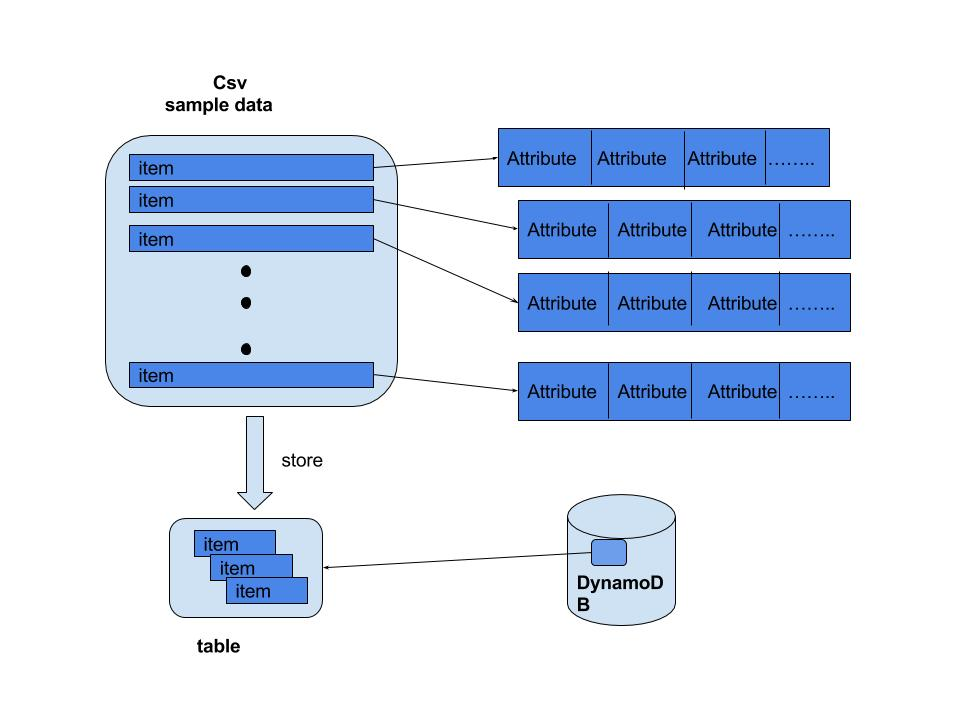
\includegraphics[width=15cm, height=8cm]{11.jpg}
 \centering
 \caption{\label{fig:1}sample csv data in DynamoDB table}
 \end{figure}

    \subsection{Algorithm viewpoint}
    Algorithm viewpoint will be use to implement different operation such as create table, upload data, update table, delete table, list table, query table and scan table.\\
\\
    Design concerns\\
    The concern for this part will be how to design the algorithm for operations. Fortunately, the Amazon provides basic APIs for the operations. So we can adapt it from the Amazon document API.\\
\\  
    AWS Java SDK\\
    AWS Java SDK is actually similar with the command line prompt in Windows. We could use it to do different implementations for the table.For instance, if we need to update some items in the table, we could use the APIs in AWS Java SDK to do the updating. However, AWS Java SDK is not efficient for uploading the items.As a result, we will only use it for simple operations such as creating table, deleting table, updating table.\\
\\
	APIs for operation\\ 
 	(1) Create Tables\\
    We will use the AWS Java SDK for creating tables. The Amazon provides the Java document API for creating tables.These API will help us to create the database schema that we need.The API will first create a dynamoDB class. After that it declares a table request which contains the table name, key of table, the definitions of attributes and capacity.\\
    Here is the API\cite{w1} :\\
    \begin{lstlisting}[language=Java, caption=API for create tables]
	DynamoDB dynamoDB = new DynamoDB(new Client(new Provider()));
	ArrayList [Attribute] attribute= new ArrayList[Attribute] ();
	attribute.add(new Attribute().withAttributeName("Id").withAttributeType("N"));
  	ArrayList[Element] key = new ArrayList[Element] ();
 	key.add(new  Element().withAttributeName("Id").withKeyType(KeyType.HASH));
	CreateTableRequest request = new CreateTableRequest()
	.withTableName(table)
	......
	.withProvisionedThroughput(new ProvisionedThroughput()
	.withReadCapacityUnits(size)
	.withWriteCapacityUnits(size));
	Table table = dynamoDB.createTable(request);
	table.waitForActive();
  \end{lstlisting}
    (2) Upload Data\\
    We will use the AWS Java SDK for uploading data into schema. The Amazon provides the Java document API for uploading data.We will use these API to upload the data into the table that we create. The API will first create dynamoDB class.After that it declares a new item which contains the primary key, string set and the numbers for uploading.\\
    Here is the API\cite{w1}:\\
    \begin{lstlisting}[language=Java, caption=API for Upload data]
    Table table = dynamoDB.getTable(Name);
    try 
    Item item = new Item()
           .withPrimaryKey(Key)
           .withString(string)
           .withNumber(number)
           .withBoolean()
           ....
           .withString();
    table.putItem();
  \end{lstlisting}
    (3) Update Table\\
    We will use the AWS Java SDK for updating table. The Amazon provides the Java document API for updating table.We will use these API to update the data in the table that we create.The API will first create table class. After that it declares a new class called “provisionedthroughput” which contains the information for updating.\\
    Here is the API\cite{w1}:
      \begin{lstlisting}[language=Java, caption=API for update table]
    DynamoDB dynamoDB = new DynamoDB(new Client(
    new Provider()));
    Table table = dynamoDB.getTable(table);
    ProvisionedThroughput provisionedThroughput = new ProvisionedThroughput()
    .withReadCapacityUnits(size)
    .withWriteCapacityUnits(size);
    table.updateTable(provisionedThroughput);
    table.waitForActive();
\end{lstlisting}
    (4) Delete Table\\
    We will use the AWS Java SDK for deleting table. The Amazon provides the Java document API for deleting table. We will use these API to deleting table. The API will create table class. After that, it deletes the table which is the table need to delete.\\
    Here is the API\cite{w1}:
      \begin{lstlisting}[language=Java, caption=API for delete data]
    DynamoDB dynamoDB = new DynamoDB(new Client(
    new Provider()));
    Table table = dynamoDB.getTable(table);
    table.delete();
    table.waitForDelete();
	\end{lstlisting}
    (5) List table\\
    We will use the AWS Java SDK for listing table. The Amazon provides the Java document API for listing table.We will use these API to list the data in the table that we create.The API will first create DynamoDB class. After that it will execute the list table method for listing table.\\
    Here is the API\cite{w1}:\\
     \begin{lstlisting}[language=Java, caption=API for list table]
    DynamoDB dynamoDB = new DynamoDB(new Client(new Provider()));
    TableCollection[Result] tables = dynamoDB.listTables();
    Iterator[Table] iterator = tables.iterator();
    while (iterator.hasNext()) 
    Table table = iteratornext();
    System.out.println(table.getTableName());
    \end{lstlisting}
    (6) Query table \\
    We will use the AWS Java SDK for query the table. The Amazon provides the Java document API for querying the table.We will use these API to query the table that we create. The API will first create DynamoDB class.Then, it will create a table class which use to represent the table for retrieving. After that, it will use the query to retrieving the data.\\
    Here is the API\cite{w2}:
      \begin{lstlisting}[language=Java, caption=API for query table]
    DynamoDB dynamoDB = new DynamoDB(
    new Client(new Provider()));
    Table table = dynamoDB.getTable(table);
    QuerySpec spec = new QuerySpec()
    .withValueMap(new ValueMap()
    ItemCollection[Query] items = table.query(spec);
    Iterator[Item] iterator = items.iterator();
    Item item = null;
    while (iterator.hasNext()) {
    item = iterator.next();
    System.out.println(item.toJSONPretty());
	\end{lstlisting}
    (7) Scan Table \\
    We will use the AWS Java SDK for scan the table.The Amazon provides the Java document API for scan the table.We will use these API to scan the table in order to read the data which store in the table. The API will create a class called “Client”. Then, it create a class which use to provide the information of table for scanning.\\
    Here is the API for Scan Table\cite{w3}:
      \begin{lstlisting}[language=Java, caption=API for scan table]
    AmazonDynamoDBClient client = new Client(
    new Provider());
    ScanRequest scanRequest = new ScanRequest()
    .withTableName(table);
    ScanResult result = client.scan(Request);
    for (Map[String, Attribute] item : result.getItems()){
    printItem(item);}
    \end{lstlisting}

 \section{Quicksight}
    \subsection{Overview}
    The data store in the DynamoDB will be used to create an analyze and a visual on Amazon visualization tool called Quicksight. In this part, Information viewpoint will be used.
    \subsection{Information viewpoint}
    The information viewpoint can be used to achieve visualization part. Basically, we will use the Quicksight as the visualization tool to represent the analyzing result.\\
\\
    Design concern \\
    The major concern for this part will be how to generate a visual on the Quicksight. Fortunately, the Amazon provides tutorial on the Quicksight document. Therefore, we can a follow the instruction step by step from the document.\\
\\    
    Step for creating a visual\\
    Base on the Quicksight document, there will be several general step for creating a visual. The first step is to create a data source in your database. These data source are very important for Quicksight because it will require these data source for creating data set and do the analyzing. After that, the Quicksight needs to connect with the data source. In this step, if the database is on the Amazon web services the data source will be easily to connect. However, if the data source is not on the Amazon web services it requires port, database access information to connect the data source in database. The detail information is on the Amazon Quicksight document. The next step is to create the data set according to data source and do an analyzing. The last step is to create a visual according to the data set. There are different types of visual on the Quicksight and we can choose one to generate the suitable graph for the analyzing result.\cite{w4}For our project, the QuickSight will get the data source and create the data set from S3 or Local PC.\\
    The figure \ref{fig:2} shows the general process:
    \begin{figure}[h]
    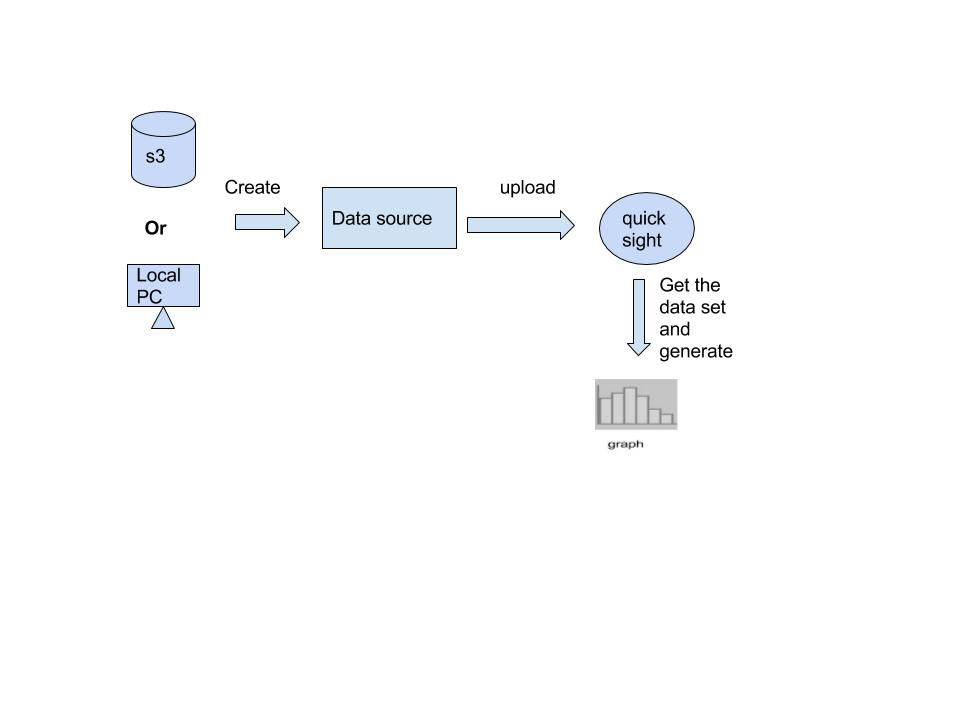
\includegraphics[width=16cm, height=7cm]{6.jpg}
    \centering
    \caption{\label{fig:2}General process}
    \end{figure}



\newpage
        \thispagestyle{empty}
        \noindent\begin{tabular}{ll}
        \makebox[2.5in]{\hrulefill} & \makebox[2.5in]{\hrulefill}\\
        Client & Date\\[8ex]% adds space between the two sets of signatures
        \makebox[2.5in]{\hrulefill}\\
        Developer 1\\[8ex]
        \makebox[2.5in]{\hrulefill}\\
        Developer 2\\[8ex]
        \makebox[2.5in]{\hrulefill}\\
        Developer 3\\[8ex]
        \end{tabular}
\end{document}
